% !TeX spellcheck = en_GB
\chapter{Background}

This section introduces concepts and techniques essential to this thesis. First, I will explain how fluorescence arises from discrete molecular energy states. Then, I will explain how the wave nature of light limits the resolution of a microscope by limiting the size of the focal spot to roughly half the wavelength of the light used, and two methods to get around it. The first method, STED microscopy, uses targeted quenching of fluorescent molecules (also called dyes or fluorophores) at the edge of the focal spot to effectively narrow down the spot size. The second method exploits the polarisation state of excitation or emission light to measure the orientation of certain structures in a sample, even if their size is below the resolution limit.

\section{Diffraction-limited fluorescence microscopy}

In short, fluorescence is a phenomenon in which a molecule absorbs a photon of one wavelength, spends a short amount of time (a couple of nanoseconds) in an excited energy state, and then emits a photon of a wavelength longer than the first one. The difference in wavelength is essential to perform microscopy, and the fact that molecules have discrete energy states is key  to generate that difference.

\begin{figure}
	\centering
	 \includegraphics[height=.4\linewidth]{jablonski diagram.ai} \hfill 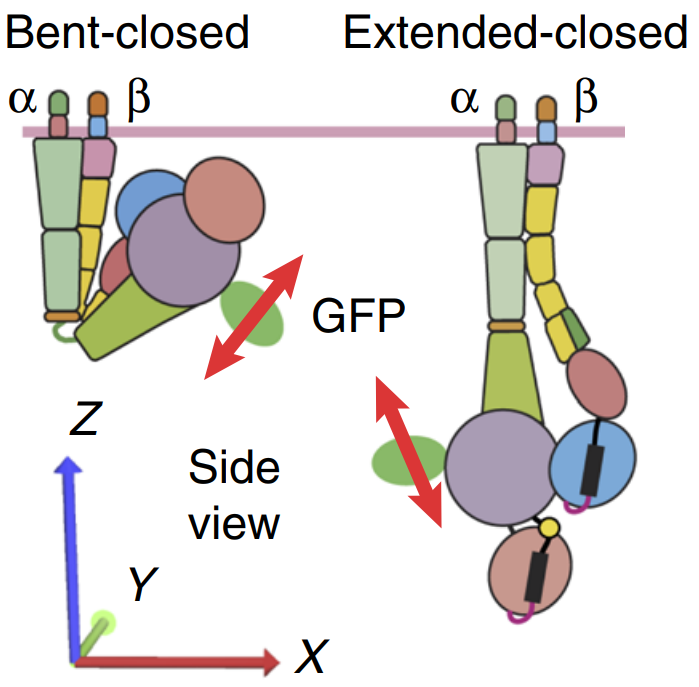
\includegraphics[height=.4\linewidth]{nordenfelt et al.png}
	\caption{
		\textbf{Left:} Illustration of the discrete energy states of a molecule and some possible transitions between them. The difference between energy levels determines the wavelength and colour of the absorbed or emitted photon. $ S_1 $ and $ S_2 $ are electronic energy levels that each contain a set of vibrational states. \textbf{Right:} Illustration of how a fluorophore's dipole moment (red arrow) can report on the orientation of the molecule it is bound to. In this case, the fluorophore is GFP (green fluorescent protein) and the target is a transmembrane integrin protein with subunits $ \alpha $ and $ \beta $. Image by Nordenfelt et al.~\cite{Nordenfelt2017}.
	}
	\label{fig:jablonski}
\end{figure}

Let us consider a molecule with two electronic energy states, each of which has a number of vibrational energy levels as in \autoref{fig:jablonski}. When the molecule is in its ground state (the lowest available energy level, $ S_0 $), it can absorb photons only if the energy they carry matches the difference between the ground state and another energy level. From an excited state ($ S_1 $), the system can relax into lower vibrational levels without emitting radiation, after which it emits a photon, relaxing back to the ground state. Two possible paths are shown in the figure. Because some energy is lost in a non-radiative way, the emitted photons will carry less energy than the absorbed photon, resulting in the wavelength difference mentioned before. This is called the Stokes shift. 

We can make that a little more rigorous by considering what happens to a simple, two-level quantum system such as a hydrogen atom subject to a Hamiltonian $ H_0 $. Denote the energy states of the electron with $ \ket{1} $ and $ \ket{2} $ (we are not taking into account vibrational levels here). These are eigenstates of the Hamiltonian with energy $ \epsilon_i $. When exposed to an electric field $ \vb{E} = \vb{E}_0 \cos\omega t$, the Hamiltonian is perturbed: $ H' = H_0 + \vb*{\mu} \cdot \vb{E}(t) $, where $ \vb*{\mu} = -e\vb{r}$. If the system is in the ground state at time $ t=0 $, the probability to find the system in the excited state at time $ t $ is given by
\begin{equation}
	\abs{c_2(t)}^2 = \abs{\mel{2}{e^{-iHt/\hbar}}{1}}^2.
\end{equation}
For weak fields, the first-order approximation is
\begin{equation}
	\abs{c_2(t)}^2 = \abs{ \frac{\vb*{\mu}_{21}\cdot\vb{E}_0}{\hbar}  \frac{\sin((\omega_0-\omega)t/2)}{\omega_0-\omega}}^2,
	\label{eq:transition moment}
\end{equation}
where $ \vb*{\mu}_{21} = \mel{2}{\vb*{\mu}}{1} $ and $ \omega_0 = (\epsilon_2-\epsilon_1)/\hbar $. More detail can be found in C.J.~Foot \cite{Foot}. From this equation, we can conclude that there are two conditions for a transition. Firstly, the frequency of the electric field must match the energy difference between the states. (Note that we have not made any statement about the sign of $ \omega_0 $. This process can represent absorption as well as stimulated emission.) Secondly, the electric field is most effective at driving the transition when it is polarised along the transition dipole moment $ \vb*{\mu}_{21} $. For example, if an electron is confined to a chemical bond, it will not interact with electric fields polarised orthogonal to that bond.The precise energy levels available depend on the molecule and its environment. Therefore, every fluorescent molecule has a unique absorption and emission spectrum, which needs to be considered when planning a fluorescence experiment.

The resolution of fluorescence microscopy used to be limited by light diffraction. Consider the diffraction limit in one of the simplest possible setups: an epifluorescence microscope. Epifluorescence microscopy is fairly similar to bright field microscopy; it is just using excitation light of a well-defined wavelength instead of white light. The sample, which is stained with a fluorescent dye, is illuminated at a wavelength that dye can absorb. The dye molecules will then emit photons of longer wavelengths in their emission spectrum, which are collected by the microscope objective. Before imaging by a CCD camera, the scattered laser light can be filtered away using a dichroic mirror that passes emission light and reflects excitation light. 


It used to be the case that microscopes were limited in resolution by the quality of their lenses and the pixel density of the CCD, but there is a much more fundamental limit, first described by Ernst Abbe. This limit is caused by the presence of an aperture. When a beam of light goes through an aperture of finite size, such as a lens, it cannot be focused onto an infinitesimal point. Instead, it will generate a spot with a radius approximately equal to $ \lambda/2\na $, where $ \lambda $ is the wavelength of the light and $ \na= n\sin\theta $ is the numerical aperture, the product of the index of refraction and the sine of the half-cone angle of the acceptance cone.

\begin{figure}[!t]
	\centering
	\begin{tabularx}{\linewidth}{lXl}
		\toprule
		& Criterion                                                                            & Definition                            \\ \midrule
		Rayleigh & The first minimum of one point's Airy function coincides with the maximum of another & $ d_{xy} = .61\lambda/\na $           \\
		FWHM     & The width of the Airy function at half of the peak height                            & $ d_{xy} = .51\lambda/\na $           \\
		Abbe     & Resolving all groups of the 19-group Norbert plate \cite{Abbe1873, Norbert}                                  & $ d_{xy} = \phantom{1}.5\lambda/\na $ \\
		Sparrow  & The distance between fluorophores at which the central maximum splits                & $ d_{xy} = .47 \lambda/\na $          \\ \bottomrule
	\end{tabularx}
	\captionof{table}{Some common definitions of the resolution limit $ d_{xy} $.}
	\label{tab:resolution limits}
	
	\centering
	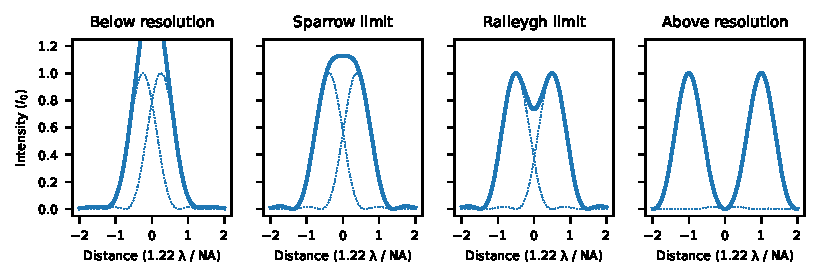
\includegraphics{diffraction_limit.pdf}
	\captionof{figure}{
		Illustration of the diffraction limit. Below the resolution limit, two fluorophores (with PSF dashed) appear under a microscope as a single peak (solid, sum of the intensities of the two fluorophores). Distance is measured in multiples of the Rayleigh limit ($ .61\lambda/\na $).
	}
	\label{fig:diffraction limit}
\end{figure}

In particular, a circular aperture will convert point sources in the sample plane to Airy patterns in the image plane. Mathematically, this can be described by a convolution product between the point spread function (PSF) $ h_\mathit{det} $ and the fluorophore distribution $ \rho $,
\begin{equation}
	I(\vb{x}) = (h_\mathit{det} * \rho)(\vb{x}) \coloneqq \int\dd{\vb{x}'} h_\mathit{det}(\vb{x}-\vb{x}')\rho(\vb{x}'),
	\label{eq:convolution}
\end{equation}
where the triple integration over the three components of $ \vb{x}' $ is implied, resulting in an image $ I(\vb{x}) $. When two fluorophores are close enough together that their PSFs overlap, they appear as a single object instead of two separate ones. This happens when the distance between them is around $ \lambda/2\na $, and that is what determines the resolution of a microscope. The exact resolution depends on your definition of this minimum resolvable distance. There are several definitions, but they are all proportional to $ \lambda/\na $. Some of them are listed in \autoref{tab:resolution limits} and visualised in \autoref{fig:diffraction limit}.



For a long time, physicists thought this limit was practically unavoidable \cite{McCutchen1967}, but in the next sections, I will discuss two ways in which one can get information from a system below the resolution limit. The first method (STED microscopy) directly increases the image resolution. The excitation light is still subject to the Abbe limit, but we add another laser to effectively improve our focusing. The second is indirect and requires playing with a new aspect of light (polarisation) that allows you to get orientational information about structures that are otherwise below the resolution limit.

\section{Super-resolution microscopy}

\begin{figure}
	\centering
	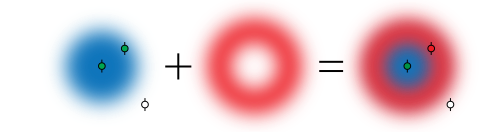
\includegraphics[width=\linewidth]{sted.ai}
	\caption{
		Working principle of STED microscopy. Fluorophores at the edge of the excitation PSF are quenched by stimulated emission, effectively resulting in a narrower PSF. Both beams are circularly polarised. 
	}
	\label{fig:sted principle}
\end{figure}

There are several ways to increase image resolution, many of which use the photophysics of individual dyes to turn off a subset of them during imaging. Some methods do this stochastically, such as STORM (stochastic optical reconstruction microscopy) and PALM (photoactivated localisation microscopy) \cite{Mock2009, Betzig2006}. These methods activate a random subset of fluorophores, such that the average distance between them is above the resolution limit. Then they are imaged with a camera and the centres of their PSFs are estimated. The precision of that estimate scales with $ 1/\sqrt{N} $ where $ N $ is the numbers of photons collected.

On the other hand, there are targeted techniques such as STED (stimulated emission depletion), GSD (ground state depletion), RESOLFT (Reversible saturable optical fluorescence transitions), and more \cite{Klar2000, Folling2008, Hofmann2005}. Generally, they work by turning off fluorophores on the outer edge of the focal spot (depletion). The resolution achieved is dependent on the intensity of the depletion laser. This is a case of targeted instead of stochastic photoswitching. The Tegenfeldt group own a STED microscope, so that is what I will focus on in this section. 

In essence, a STED microscope is a scanning confocal microscope with an extra laser that can selectively deplete fluorescence by stimulated emission. Its working principle is shown in Figures \ref{fig:sted principle} and \ref{fig:sted microscope}. In a scanning confocal microscope, the excitation laser does not illuminate the whole sample at once, but is scanned over it. This means only fluorophores in an Airy disk around the focus will be excited. Furthermore, the detector is now comprised of a pinhole and a photodetector (not a camera), which filters out most of the out-of-focus light \cite{Minsky1957}. Therefore, the PSF of a confocal microscope is the product of the laser PSF $ h_\exc $ and the detection probability $ h_\mathit{det} $
\begin{equation}
	h_\mathit{conf}(\vb{x}) = h_\exc(\vb{x}) \cdot h_\mathit{det}(\vb{x}),
\end{equation}
where the most important characteristic of $ h_\mathit{det}(\vb{x}) $ is that it is quite narrow in the $ z $ direction. The smaller the detection pinhole, the stronger this effect. However, a smaller detection pinhole also means that even a fraction of the light from the focal plane will be rejected from the photodetector. Therefore, there is a trade-off between $ z $ resolution and the signal-to-noise ratio (SNR).

Even though both of these PSFs are diffraction-limited, a STED microscope can reach an arbitrarily small resolution \cite{Wildanger2012}. It does so by illuminating the sample with a donut-shaped laser at a wavelength longer than the emission wavelength. Referring back to \autoref{fig:jablonski}, the blue laser excites the fluorophores that emit in green, but a red transition is also allowed. Under illumination with a red laser, this transition is made more favourable by the process of stimulated emission, first postulated by Einstein in 1926 \cite{Einstein1926}. This way, fluorophores at the edge of the excitation PSF can be prevented from emitting green light, while fluorophores at the centre do not experience stimulated emission, which reduces the width of the effective point spread function. An illustration of this effect is given in \autoref{fig:sted principle}.


More rigorously, the STED beam depletes fluorescence according to
\begin{equation}
	\eta(\vb{x}) = \exp(-\sigma_\dep h_\dep(\vb{x})),
\end{equation}
which relates the fraction of fluorescence remaining as a function of the depletion intensity $ h_\dep $. Therefore, the STED point spread function can be expressed as
\begin{equation}
	h_\mathit{STED} = h_\exc(\vb{x}) \cdot \eta(\vb{x}) \cdot h_\mathit{det}(\vb{x}),
\end{equation}
which can be read as ``the probability for a dye to be excited, times the probability for it not to be quenched by stimulated emission, times the probability for fluorescence emission to be detected by the CCD''. Even though every individual PSF ($ h_\exc(\vb{x}) $, $ h_\dep(\vb{x}) $ and $ h_\mathit{det}(\vb{x}) $) is diffraction-limited, the fact that you need to multiply them results in a narrowing of the effective PSF below the Abbe limit. This means that the extent of the resolution improvement depends on the intensity of the depletion laser $ I_\dep$. Harke et al.~approximate the STED resolution as
\begin{equation}
	d_\mathit{STED} = \frac{d_c}{\sqrt{1+d_c^2a^2\cfrac{I_\dep}{I_\mathit{sat}}}},
\end{equation}
where $ d_c $ is the resolution limit of a confocal microscope, $ a $ the steepness of the donut pattern (i.e.~high $ a $ means very tight central minimum in the donut-shaped intensity), and $ I_\mathit{sat} $ is the depletion intensity at which fluorophore brightness is reduced by half \cite{Harke2008}.

\begin{figure}
	\centering
	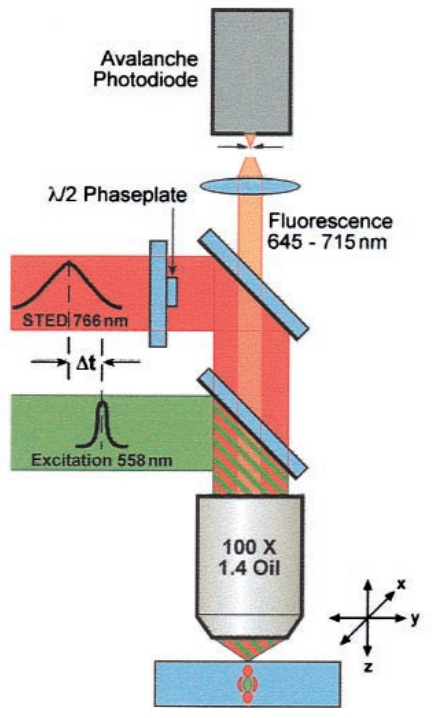
\includegraphics[width=0.3\linewidth]{sted microscope schematic.png}
	\caption{
		The rough layout of a STED microscope. The excitation laser is focused on the sample, and the STED laser forms a donut pattern around the focal spot. Emitted light is collected by the objective and focused on a pinhole before it is detected by an APD. Figure from Klar et al.~2000 \cite{Klar2000}.
	}
	\label{fig:sted microscope}
\end{figure}

Although STED can reach an arbitrary resolution under optimal circumstances, the resolution reached in biological specimens is more usually around 50~nm \cite{Wildanger2012,Muller2012}. If information is desired at an even smaller scale using fluorescence microscopy, then other methods are required.
There are several reasons the resolution of STED in biological samples has not been able to reach the single-nanometre scale. One is that these samples consist of cells in a water-based solution, which causes a strong mismatch in the index of refraction between the sample and the optics used (commonly glass and oil). Another is the limited photostability of the dyes. Every time a fluorophore absorbs a photon, there is a probability that a photochemical event occurs that damages (bleaches) the fluorophore. Good fluorophores can typically absorb 10 000 to 40 000 photons before this happens \cite{Lichtman2005}. Therefore, high excitation powers result in high bleaching rates. Photobleaching is mainly due to interactions with reactive oxygen species and is therefore not only determined by the properties of the fluorophore, but also the environment. Photobleaching can also be induced by other causes, such as the absorption of multiple photons. Refer to Diaspro et al.~for an overview of photobleaching \cite{Diaspro2006}. When imaging live cells, phototoxicity also needs to be taken into account. Because molecules other than the targeted fluorophores can also absorb laser light (possibly resulting in autofluorescence), incident radiation can be toxic for the cell, for the same reasons as it can bleach a fluorophore \cite{Lichtman2005}. Therefore, photobleaching and phototoxicity both limit the laser power that can be applied.


\section{Polarisation microscopy}

Polarisation microscopy uses the vectorial nature of light -- the fact that light consists of electromagnetic waves that with a certain polarisation -- to get orientational information of fluorophores below the resolution limit. Other methods to get information on distances below the resolution limit  include fluorescence resonance energy transfer (FRET) \cite{Lerner2021}, for example, which is great for measuring distances between two fluorophores on the order of nanometres.

Among others, light polarisation microscopy has been used to measure how the structure of DNA changes when it is subject to a strong stretching force, how integrin proteins respond to an applied force and the order of molecules embedded in the cell membrane \cite{Backer2019, Nordenfelt2017, Swaminathan2017, Brasselet2013}. In this section, I will first introduce the concept of light polarisation, then discuss how it can be used in a microscope, and finally mention some optical components that affect the light polarisation, which are crucial to conducting a polarisation microscopy experiment. For a more exhaustive introduction to polarisation microscopy, there are several good resources available \cite{Goldstein2011, Collett2005, Lakowicz2006}.

\subsection{The polarisation ellipse.} Light is a transverse electromagnetic wave, meaning that there are oscillations of the electric and magnetic fields along the path of a light ray, and that these oscillations are orthogonal to the propagation direction. In other words, if the light propagates along $\vb{k}$, the electric and magnetic fields $\vb{E}$ and $\vb{B}$ must satisfy $ \vb{E} \cdot \vb{k} = \vb{B} \cdot \vb{k} = 0$. (The fields themselves are also orthogonal to each other, so we can neglect $ \vb{B} $ without compromising our analysis.)

For the sake of simplicity, let us consider a ray propagating in the $ z $ direction. The electric field at any point in space and time can be written as
\begin{align}
	E_x(z, t) &= \Eox \cos(kz-\omega t + \phi_x),\\
	E_y(z, t) &= \Eoy \cos(kz-\omega t + \phi_y).
\end{align}
where $ \vb{E}_0 $ is the amplitude of the oscillation, $ k $ is the wavenumber (the length of $ \vb{k} $), $ \omega $ is the radial frequency and $ \phi $ is an arbitrary phase. Note that the wavenumber and the frequency are related to each other through the speed of light $ c $, since $ \omega = kc = \hbar c/\lambda$. Note also that the $ x $ and $ y $ components can have a phase difference.

Letting $ \delta = \phi_y-\phi_x $, it can be shown that 
\begin{equation}
	\left(\frac{E_x}{\Eox}\right)^2 - 2\cos\delta\frac{E_x}{\Eox}\frac{E_y}{\Eoy} + \left(\frac{E_y}{\Eoy}\right)^2 = \sin^2\delta,
\end{equation}
which is the equation for an ellipse. This means that at any point in time, the point $ (E_x, E_y) $ lies on the ellipse defined by the equation above, which is called the polarisation ellipse and is completely determined by $ \Eox $, $ \Eoy $ and $ \delta $. Together, these values determine whether the polarisation is linear, circular, or something in between. Refer to \autoref{tab:polarisation states} for an overview.

\begin{table}
	\centering
	\begin{tabular}{lcccc}
		\toprule
		Polarisation state      & $ \Eox $ & $ \Eoy $ & $ \delta $ &     Jones vector      \\ \midrule
		Linear along $ x $      &    1     &    0     &    any     & $ (1, \phantom{-}0) $ \\
		Linear along $ y $      &    0     &    1     &    any     & $ (0, \phantom{-}1) $ \\
		Linear at \ang{+-45}    &    1     & $ \pm1 $ &     0      &     $ (1, \pm1) $     \\
		Circular (right-handed) &    1     &    1     & $ \pi/4 $  & $ (1, \phantom{-}i) $ \\
		Circular (left-handed)  &    1     &    1     & $ -\pi/4 $ &      $ (1, -i) $      \\ \bottomrule
	\end{tabular}
	\caption{List of a number of polarisation states (not normalised).}
	\label{tab:polarisation states}
\end{table}


In general, the polarisation ellipse can be defined by means of two angles: the orientation $ \psi $ and ellipticity $ \chi $, as shown in \autoref{fig:pol ellipse}. They can be calculated from $ \alpha = \arctan(\Eoy/\Eox) $ and the phase difference $ \delta $ using
\begin{align}
	\tan 2\psi &= \tan 2\alpha \cos \delta,\\
	\sin 2\chi &= \sin 2\alpha \sin \delta
\end{align}
This definition of $ \chi $ is dependent on the ratio of the maximum and minimum amplitude of the electric field as is presented in \autoref{fig:pol ellipse}. One can define a similar value based on the corresponding intensities. Since $ I = \abs{\vb{E}_0}^2 $,
\begin{align}
	\chi_I &= \arctan {I_\mathit{max}}/{I_\mathit{min}} = \arctan\left[ \left( {E_\mathit{max}}/{E_\mathit{min}} \right)^2 \right] .
\end{align}
To distinguish between them, I will be using $ \chi_E $ and $ \chi_I $ from now on. These are useful concepts because they are relatively easy to calculate from intensity measurements. Therefore, I will use them when I characterise laser beams in the setup.

\begin{figure}
	\centering
	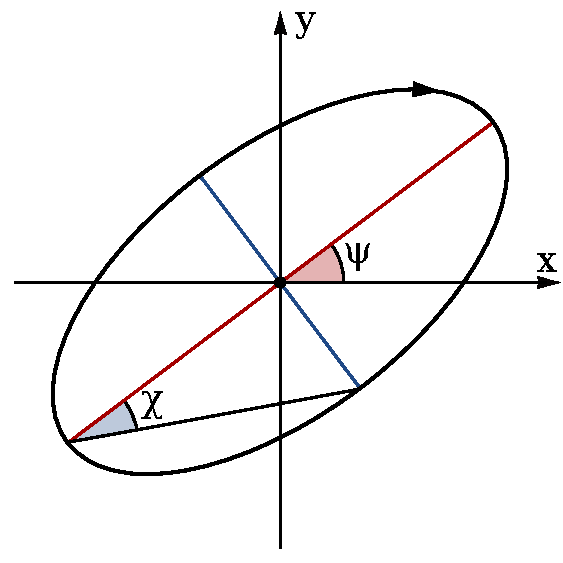
\includegraphics[width=.3\linewidth]{polarisation_ellipse.pdf}
	\caption{The meaning of $ \psi $ and $ \chi $ in the context of the polarisation ellipse. (Figure by Wikipedia user Inductiveload)}
	\label{fig:pol ellipse}
\end{figure}

\subsection{Microscopy.} Why is polarisation relevant to microscopy? Well, the probability of excitation is dependent on the polarisation of incoming light. Since a fluorophore can be considered a small dipole moment, it will not interact with radiation that is orthogonal to the transition dipole moment of the fluorophore (see discussion around \autoref{eq:transition moment}). If the excitation laser is polarised along an angle $ \psi $ and the dipole is oriented along $ \theta $, the intensity of light emitted by that fluorophore will satisfy 
\begin{equation}
	\label{eq:malus}
	I(\psi, \theta) \propto \cos^2(\psi-\theta).
\end{equation}
This is Malus's law. Analogously, light emitted from a fluorophore is always linearly polarised parallel to the transition dipole moment. One can place a linearly polarising filter in front of the detector to measure a fluorophore's orientation. If the polariser emits light polarised at an angle $ \psi $, then the intensity measured at the detector also follows Malus's law, meaning that these two setups are analogous (not taking into account depolarisation effects in an experimental setup). As an example, see \autoref{fig:composite}. Dipole excitation by circularly polarised light is usually not dependent on $ \theta $, but there are fluorophores that are sensitive to the handedness of circularly polarised light \cite{Takaishi2019}.

Common polarisation microscopy protocols include: rotating a linearly polarised excitation laser, rotating a polarising filter in the excitation beam path, or doing both. The first polarisation measurements were done by excitation of the sample with a linearly polarised laser and measuring the fractions of emission intensity that were parallel and orthogonal to the excitation light. With those, one can calculate the anisotropy of a sample \cite{Camacho2019}. I will elaborate on different polarisation microscopy methods in \autoref{sec:pol analysis}. 

\subsection{Jones calculus.} Lasers are usually linearly polarised, but I have not yet mentioned how we can manipulate this polarisation to run the experiments we want. There are optical elements such as waveplates that can do this for us, and the best way to understand them is through Jones calculus. This is an incredibly useful way to model light polarisation, but it does require us to express the electric field as a complex function:
\begin{equation}
	\vb{E}(z, t) = \vb{E}_0 e^{i(kz-\omega t)}.
	\label{eq:propagator}
\end{equation}
In the following analysis, we will treat $ \vb{E} $ as a two-dimensional vector with only an $ x $ and $ y $ component, since $ E_z = 0 $. Note that complex numbers are just a mathematical trick. The Maxwell equations that govern light propagation are linear, and taking the real part of a complex-valued function is also a linear operation, so the complex extension of $ \vb{E} $ will behave exactly like the actual electric field would. The phase difference between the two components is now contained in $ \vb{E}_0 $, which can be expressed as
\begin{equation}
	\vb{E}_0 = \mqty(\Eox \\ \Eoy e^{i\delta} ).
\end{equation}
The Jones vectors for some special polarisation states are listed in \autoref{tab:polarisation states}.

The usefulness of Jones calculus lies in its ability to represent optical components as matrices acting on this vector. For example, a polariser that transmits $ x $-polarised light has the following matrix form:
\begin{equation}
	S_p = \mqty(1 & 0 \\ 0 & 0).
\end{equation}
It is easy to verify that $ S_p \vb{E}_0 = \Eox $. We also need to take into account how mirrors affect polarisation. In this case, it is useful to define a new coordinate system. Let $ k $ be the propagation direction, $ p $ the direction that is orthogonal to $ k $, but in the plane of incidence: the plane formed by $ k $ and the normal to the mirror surface (i.e. $ p $ is parallel to the plane of incidence). Finally, let $ s $ be orthogonal to $ k $ and $ p $ ($ s $ stands for the German word senkrecht). A mirror flips the $ s $ component of the field polarisation, while keeping $ p $ unchanged. So, a mirror whose surface is parallel to the $ x $-axis has a Jones matrix of the form
\begin{equation}
	S_{mx} = \mqty(1 & 0 \\ 0 & -1).
\end{equation}

Another important type of optical component in our setup is a waveplate. Waveplates or phase retarders are made out of birefringent crystals such as quartz, meaning the index of refraction a ray of light experiences is dependent on its polarisation. This happens when a crystal structure lacks cubic symmetry. When the coordinate system is aligned with the crystal axes, we might find that $ k_x = k_z = k_o $ (the ordinary axes), while $ k_y = k_e $ (the extraordinary axis). $ k_e $ may both be greater or less than $ k_o $. In these crystals, \autoref{eq:propagator} is no longer valid and should be replaced by
\begin{equation}
	\vb{E}(z, t) = \mqty(\Eox e^{i(k_o z-\omega t)} \\ \Eoy e^{i(k_e z-\omega t + \delta)} ).
\end{equation}
This can also be written in the form
\begin{equation}
	\vb{E}(z, t) = \mqty(\Eox  \\ \Eoy e^{i(\Gamma(z) + \delta)} ) e^{i(k_o z-\omega t)}
	\qq{, where}
	\Gamma(z) = (k_e-k_0) z.
\end{equation}
As one can see, a waveplate only imparts a delay on the $ y $-component of a beam, depending on its thickness $ z $ and its birefringence. We can neglect the phase factor common to both components and represent the action of a waveplate by the following Jones matrix in the local coordinate system of the waveplate with
\begin{equation}
	S_\Gamma = \mqty(1 & 0 \\ 0 & e^{i\Gamma}).
\end{equation}
We can name the axes in this coordinate system the fast and slow axes, where the field component along the slow axis incurs the phase delay.

Generally, waveplates are characterised by the relative delay they impart on polarisation components. Quarter-wave plates delay it by a quarter of a wavelength compared to the fast propagating ray, corresponding to $ \Gamma = (2n + 1/2)\pi $ (for any integer $ n $). Therefore, the Jones matrix of a quarter-wave plate satisfies 
\begin{equation}
	S_\qwp = \mqty(1 & 0 \\ 0 & e^{i\pi/2}) = \mqty(1 & 0 \\ 0 & i).
\end{equation}
Let's consider what happens to some specific cases. If vertically or horizontally polarised light passes through a quarter-wave plate, its polarisation will not change. But light polarised along $ +\ang{45} $ ($ -\ang{45} $) will be turned into left-handed (right-handed) light, and vice versa. Therefore, a quarter-wave plate allows us to convert between linearly and circularly polarised light, as shown in \autoref{fig:waveplates}.

\begin{figure}
	\centering
	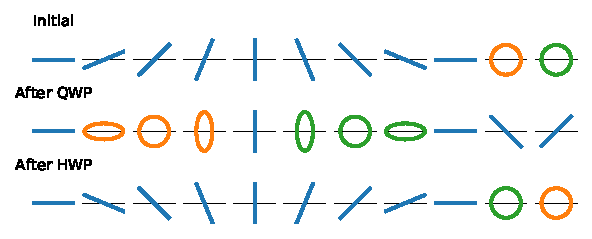
\includegraphics{waveplates.pdf}
	\caption{
		The effect of quarter-wave plates (QWP) and half-wave plates (HWP) on the polarisation ellipse. The fast axis is horizontal and indicated in the figure. The slow axis is vertical. Orange: left-handed polarisation. Green: right-handed polarisation. The ray is propagating into the page.
	}
	\label{fig:waveplates}
\end{figure}

The second type of waveplate we should treat is a half-wave plate. It features a delay of $ \Gamma = (2n+1)\pi $, and its Jones matrix looks like
\begin{equation}
	S_\hwp = \mqty(1 & 0 \\ 0 & e^{i\pi}) = \mqty(1 & 0 \\ 0 & -1),
\end{equation}
which corresponds to mirroring the polarisation state along the $ x $-axis. Another way to think about it is that a ray polarised along an angle $ \psi $ will be rotated by an angle $ -2\psi $, and the handedness of circularly polarised light will be reversed, see \autoref{fig:waveplates}.

The power of Jones calculus lies in its ability to model the behaviour of a sequence of optical elements at arbitrary rotations. First, we need to define the Jones matrix for a rotated component. This is simply
\begin{equation}
	S(\theta) = R(\theta) \cdot S \cdot R(-\theta),
	\qq{where} 
	R(\theta) = \mqty(\cos\theta & -\sin\theta \\ \sin\theta & \cos\theta)
\end{equation}
and $ \theta $ is the angle of the component's fast axis with the lab coordinate system's $ x $ axis. As an example, we can send $ x $ polarised light through a polarising filter at an angle $ \theta $, which results in
\begin{equation}
	I(\theta) \propto \abs{S_p(\theta) \cdot \mqty(1 \\ 0)}^2 = \cos^2\theta.
\end{equation}
That is Malus's law, as we had defined before. We can also recover the same behaviour by using a fixed polarising filter and a half-wave plate at an angle $ \theta/2 $:
\begin{equation}
	I(\theta) \propto \abs{S_p(0) \cdot S_\hwp(\theta/2) \cdot \mqty(\admat{1 \\ 0})}^2 = \cos^2\theta.
\end{equation}

Jones calculus has its limitations, the main one being that it cannot represent unpolarised light (an incoherent sum of different polarisations). Müller calculus, based on real-valued 4D Stokes vectors instead of the complex 2D Jones vectors, can handle it. As such, Müller calculus can also quantify depolarisation induced by non-ideal microscope optics. In this thesis, I mainly used Jones calculus to develop a theoretical understanding of the optical elements in the STED microscope, so using Müller matrices was not necessary. In the next sections, I will use the theory presented here to implement polarisation microscopy on the Tegenfeldt STED microscope. I will even develop the theory further to extend the concept of the optical point spread function into polarisation space.
